\section*{Informations générales}
 
\begin{table}[H]
\centering
	\begin{tabularx}{16.8cm}{|X|X|}
	\hline
	\rowcolor{gray!40} Numéro de l'opportunité & Type de l'opportunité \\
	\hline
	 002 & Livrable terminé en avance  \\
	\hline
	\end{tabularx}
\end{table}

\begin{table}[H]
\centering
	\begin{tabularx}{16.8cm}{|X|X|X|}
	\hline
	\rowcolor{gray!40} Date & Visa du \RQ & Visa du \CP \\
	\hline
	 29/01/2016 & pgpic & pgpic \\
	\hline
	\end{tabularx}
\end{table}

\begin{table}[H]
\centering
	\begin{tabularx}{16.8cm}{|X|X|X|X|}
	\hline
	\rowcolor{gray!40} Pilote & Activité WBS & Compte WBS & Phase d'apparition \\
	\hline
	 \Kafui & Suivre les Risques et Opportunités & 1.2.3.2 & Fin de Sprint \\
	\hline
	\end{tabularx}
\end{table}

\section*{Description de l'opportunité}

\subsection*{Résumé}
	Le livrable disponible à l'avance permettrait de passer directement à la phase de recette. Ceci permettrait de réinvestir le temps gagné dans une autre phase.
	
\subsection*{Analyse des causes}
	
Voir figure \ref{opportunite livrable termine en avance}.

\subsection*{Criticité}

\begin{table}[H]
\centering
	\begin{tabularx}{16.8cm}{|>{\columncolor{gray!40}}X|X|}
	\hline
	Bénéfice & 4\\
	\hline
	Probabilité & 2 \\
	\hline
	Criticité & Important \\
	\hline
	\end{tabularx}
\end{table}

\newpage
\section*{Actions}
\subsection*{Actions proactives}

{\centering
	\begin{longtable}{|p{7cm}|p{7cm}|}
	\hline
	\rowcolor{gray!40}Numéro de cause & Actions proactives \\
	
	\hline
	  1 &  \begin{itemize}
	  	\item Entretien individualisé
	  	\item Bonne communication
	  	\end{itemize} \\
	  	
	  \hline
	  2 & \begin{itemize} 
	  \item Team-Building
	  \item Entretien individualisé
	  \end{itemize} \\
	  \hline
	  3 & \begin{itemize} 
	  \item Faire remonter les problématiques fréquentes rencontrées en PIC à la direction. 
	  \end{itemize} \\
	  \hline
	   4 & \begin{itemize}
	   \item Bonne communication autour du projet. 
	   \end{itemize} \\
	\hline
	
\end{longtable}}

\section*{Décision de clôture}
Par le \CP{} et le pilote du risque.
\begin{table}[h]
\centering
	\begin{tabularx}{16.8cm}{|X|X|}
	\hline
	\rowcolor{gray!40} Date de clôture & Raison de la clôture \\
	\hline
	  & \\
	\hline
	\end{tabularx}
\end{table}

\section*{Historique des modifications}
\begin{table}[h]
\centering
	\begin{tabularx}{16.8cm}{|X|X|}
	\hline
	\rowcolor{gray!40} Date & Modification \\
	\hline
	  & \\
	\hline
	\end{tabularx}
\end{table}
\newpage

\begin{figure}[!h]
	\centering
	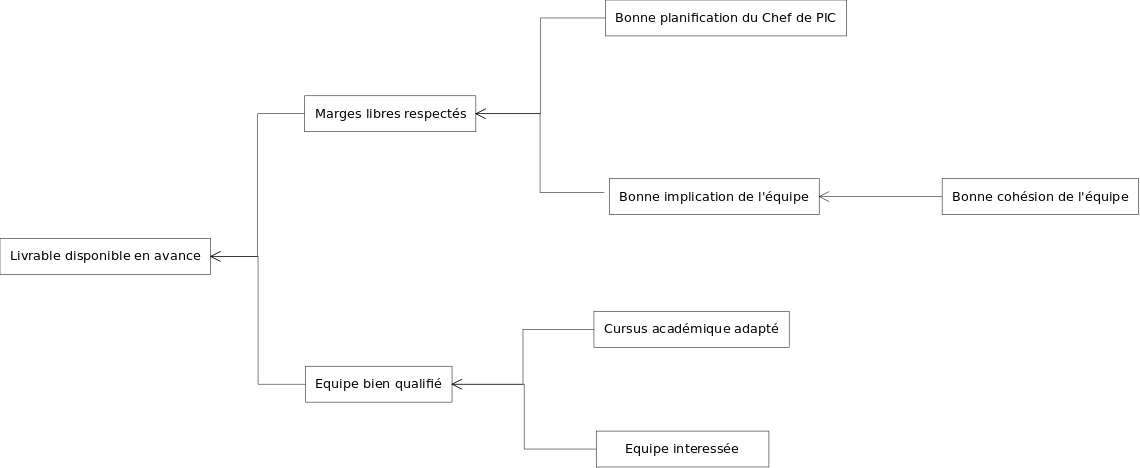
\includegraphics[scale=0.27]{images/AnalyseOpportunite_nPourquoi_FDO002}
	\caption{\label{opportunite livrable termine en avance} Opportunité livrable terminé en avance - méthode des n pourquoi}
\end{figure}
